% Options for packages loaded elsewhere
% Options for packages loaded elsewhere
\PassOptionsToPackage{unicode}{hyperref}
\PassOptionsToPackage{hyphens}{url}
\PassOptionsToPackage{dvipsnames,svgnames,x11names}{xcolor}
%
\documentclass[
  letterpaper,
  DIV=11,
  numbers=noendperiod]{scrartcl}
\usepackage{xcolor}
\usepackage{amsmath,amssymb}
\setcounter{secnumdepth}{-\maxdimen} % remove section numbering
\usepackage{iftex}
\ifPDFTeX
  \usepackage[T1]{fontenc}
  \usepackage[utf8]{inputenc}
  \usepackage{textcomp} % provide euro and other symbols
\else % if luatex or xetex
  \usepackage{unicode-math} % this also loads fontspec
  \defaultfontfeatures{Scale=MatchLowercase}
  \defaultfontfeatures[\rmfamily]{Ligatures=TeX,Scale=1}
\fi
\usepackage{lmodern}
\ifPDFTeX\else
  % xetex/luatex font selection
\fi
% Use upquote if available, for straight quotes in verbatim environments
\IfFileExists{upquote.sty}{\usepackage{upquote}}{}
\IfFileExists{microtype.sty}{% use microtype if available
  \usepackage[]{microtype}
  \UseMicrotypeSet[protrusion]{basicmath} % disable protrusion for tt fonts
}{}
\makeatletter
\@ifundefined{KOMAClassName}{% if non-KOMA class
  \IfFileExists{parskip.sty}{%
    \usepackage{parskip}
  }{% else
    \setlength{\parindent}{0pt}
    \setlength{\parskip}{6pt plus 2pt minus 1pt}}
}{% if KOMA class
  \KOMAoptions{parskip=half}}
\makeatother
% Make \paragraph and \subparagraph free-standing
\makeatletter
\ifx\paragraph\undefined\else
  \let\oldparagraph\paragraph
  \renewcommand{\paragraph}{
    \@ifstar
      \xxxParagraphStar
      \xxxParagraphNoStar
  }
  \newcommand{\xxxParagraphStar}[1]{\oldparagraph*{#1}\mbox{}}
  \newcommand{\xxxParagraphNoStar}[1]{\oldparagraph{#1}\mbox{}}
\fi
\ifx\subparagraph\undefined\else
  \let\oldsubparagraph\subparagraph
  \renewcommand{\subparagraph}{
    \@ifstar
      \xxxSubParagraphStar
      \xxxSubParagraphNoStar
  }
  \newcommand{\xxxSubParagraphStar}[1]{\oldsubparagraph*{#1}\mbox{}}
  \newcommand{\xxxSubParagraphNoStar}[1]{\oldsubparagraph{#1}\mbox{}}
\fi
\makeatother

\usepackage{color}
\usepackage{fancyvrb}
\newcommand{\VerbBar}{|}
\newcommand{\VERB}{\Verb[commandchars=\\\{\}]}
\DefineVerbatimEnvironment{Highlighting}{Verbatim}{commandchars=\\\{\}}
% Add ',fontsize=\small' for more characters per line
\usepackage{framed}
\definecolor{shadecolor}{RGB}{241,243,245}
\newenvironment{Shaded}{\begin{snugshade}}{\end{snugshade}}
\newcommand{\AlertTok}[1]{\textcolor[rgb]{0.68,0.00,0.00}{#1}}
\newcommand{\AnnotationTok}[1]{\textcolor[rgb]{0.37,0.37,0.37}{#1}}
\newcommand{\AttributeTok}[1]{\textcolor[rgb]{0.40,0.45,0.13}{#1}}
\newcommand{\BaseNTok}[1]{\textcolor[rgb]{0.68,0.00,0.00}{#1}}
\newcommand{\BuiltInTok}[1]{\textcolor[rgb]{0.00,0.23,0.31}{#1}}
\newcommand{\CharTok}[1]{\textcolor[rgb]{0.13,0.47,0.30}{#1}}
\newcommand{\CommentTok}[1]{\textcolor[rgb]{0.37,0.37,0.37}{#1}}
\newcommand{\CommentVarTok}[1]{\textcolor[rgb]{0.37,0.37,0.37}{\textit{#1}}}
\newcommand{\ConstantTok}[1]{\textcolor[rgb]{0.56,0.35,0.01}{#1}}
\newcommand{\ControlFlowTok}[1]{\textcolor[rgb]{0.00,0.23,0.31}{\textbf{#1}}}
\newcommand{\DataTypeTok}[1]{\textcolor[rgb]{0.68,0.00,0.00}{#1}}
\newcommand{\DecValTok}[1]{\textcolor[rgb]{0.68,0.00,0.00}{#1}}
\newcommand{\DocumentationTok}[1]{\textcolor[rgb]{0.37,0.37,0.37}{\textit{#1}}}
\newcommand{\ErrorTok}[1]{\textcolor[rgb]{0.68,0.00,0.00}{#1}}
\newcommand{\ExtensionTok}[1]{\textcolor[rgb]{0.00,0.23,0.31}{#1}}
\newcommand{\FloatTok}[1]{\textcolor[rgb]{0.68,0.00,0.00}{#1}}
\newcommand{\FunctionTok}[1]{\textcolor[rgb]{0.28,0.35,0.67}{#1}}
\newcommand{\ImportTok}[1]{\textcolor[rgb]{0.00,0.46,0.62}{#1}}
\newcommand{\InformationTok}[1]{\textcolor[rgb]{0.37,0.37,0.37}{#1}}
\newcommand{\KeywordTok}[1]{\textcolor[rgb]{0.00,0.23,0.31}{\textbf{#1}}}
\newcommand{\NormalTok}[1]{\textcolor[rgb]{0.00,0.23,0.31}{#1}}
\newcommand{\OperatorTok}[1]{\textcolor[rgb]{0.37,0.37,0.37}{#1}}
\newcommand{\OtherTok}[1]{\textcolor[rgb]{0.00,0.23,0.31}{#1}}
\newcommand{\PreprocessorTok}[1]{\textcolor[rgb]{0.68,0.00,0.00}{#1}}
\newcommand{\RegionMarkerTok}[1]{\textcolor[rgb]{0.00,0.23,0.31}{#1}}
\newcommand{\SpecialCharTok}[1]{\textcolor[rgb]{0.37,0.37,0.37}{#1}}
\newcommand{\SpecialStringTok}[1]{\textcolor[rgb]{0.13,0.47,0.30}{#1}}
\newcommand{\StringTok}[1]{\textcolor[rgb]{0.13,0.47,0.30}{#1}}
\newcommand{\VariableTok}[1]{\textcolor[rgb]{0.07,0.07,0.07}{#1}}
\newcommand{\VerbatimStringTok}[1]{\textcolor[rgb]{0.13,0.47,0.30}{#1}}
\newcommand{\WarningTok}[1]{\textcolor[rgb]{0.37,0.37,0.37}{\textit{#1}}}

\usepackage{longtable,booktabs,array}
\usepackage{calc} % for calculating minipage widths
% Correct order of tables after \paragraph or \subparagraph
\usepackage{etoolbox}
\makeatletter
\patchcmd\longtable{\par}{\if@noskipsec\mbox{}\fi\par}{}{}
\makeatother
% Allow footnotes in longtable head/foot
\IfFileExists{footnotehyper.sty}{\usepackage{footnotehyper}}{\usepackage{footnote}}
\makesavenoteenv{longtable}
\usepackage{graphicx}
\makeatletter
\newsavebox\pandoc@box
\newcommand*\pandocbounded[1]{% scales image to fit in text height/width
  \sbox\pandoc@box{#1}%
  \Gscale@div\@tempa{\textheight}{\dimexpr\ht\pandoc@box+\dp\pandoc@box\relax}%
  \Gscale@div\@tempb{\linewidth}{\wd\pandoc@box}%
  \ifdim\@tempb\p@<\@tempa\p@\let\@tempa\@tempb\fi% select the smaller of both
  \ifdim\@tempa\p@<\p@\scalebox{\@tempa}{\usebox\pandoc@box}%
  \else\usebox{\pandoc@box}%
  \fi%
}
% Set default figure placement to htbp
\def\fps@figure{htbp}
\makeatother





\setlength{\emergencystretch}{3em} % prevent overfull lines

\providecommand{\tightlist}{%
  \setlength{\itemsep}{0pt}\setlength{\parskip}{0pt}}



 


\KOMAoption{captions}{tableheading}
\makeatletter
\@ifpackageloaded{caption}{}{\usepackage{caption}}
\AtBeginDocument{%
\ifdefined\contentsname
  \renewcommand*\contentsname{Table of contents}
\else
  \newcommand\contentsname{Table of contents}
\fi
\ifdefined\listfigurename
  \renewcommand*\listfigurename{List of Figures}
\else
  \newcommand\listfigurename{List of Figures}
\fi
\ifdefined\listtablename
  \renewcommand*\listtablename{List of Tables}
\else
  \newcommand\listtablename{List of Tables}
\fi
\ifdefined\figurename
  \renewcommand*\figurename{Figure}
\else
  \newcommand\figurename{Figure}
\fi
\ifdefined\tablename
  \renewcommand*\tablename{Table}
\else
  \newcommand\tablename{Table}
\fi
}
\@ifpackageloaded{float}{}{\usepackage{float}}
\floatstyle{ruled}
\@ifundefined{c@chapter}{\newfloat{codelisting}{h}{lop}}{\newfloat{codelisting}{h}{lop}[chapter]}
\floatname{codelisting}{Listing}
\newcommand*\listoflistings{\listof{codelisting}{List of Listings}}
\makeatother
\makeatletter
\makeatother
\makeatletter
\@ifpackageloaded{caption}{}{\usepackage{caption}}
\@ifpackageloaded{subcaption}{}{\usepackage{subcaption}}
\makeatother
\usepackage{bookmark}
\IfFileExists{xurl.sty}{\usepackage{xurl}}{} % add URL line breaks if available
\urlstyle{same}
\hypersetup{
  pdftitle={predictors2025},
  colorlinks=true,
  linkcolor={blue},
  filecolor={Maroon},
  citecolor={Blue},
  urlcolor={Blue},
  pdfcreator={LaTeX via pandoc}}


\title{predictors2025}
\author{}
\date{}
\begin{document}
\maketitle


\begin{Shaded}
\begin{Highlighting}[]
\FunctionTok{library}\NormalTok{(forecast)}
\end{Highlighting}
\end{Shaded}

\begin{verbatim}
Warning: package 'forecast' was built under R version 4.4.3
\end{verbatim}

\begin{Shaded}
\begin{Highlighting}[]
\FunctionTok{library}\NormalTok{(tidyverse)}
\end{Highlighting}
\end{Shaded}

\begin{verbatim}
Warning: package 'tidyverse' was built under R version 4.4.3
\end{verbatim}

\begin{verbatim}
Warning: package 'ggplot2' was built under R version 4.4.3
\end{verbatim}

\begin{verbatim}
-- Attaching core tidyverse packages ------------------------ tidyverse 2.0.0 --
v dplyr     1.1.4     v readr     2.1.5
v forcats   1.0.0     v stringr   1.5.1
v ggplot2   4.0.0     v tibble    3.2.1
v lubridate 1.9.4     v tidyr     1.3.1
v purrr     1.0.2     
-- Conflicts ------------------------------------------ tidyverse_conflicts() --
x dplyr::filter() masks stats::filter()
x dplyr::lag()    masks stats::lag()
i Use the conflicted package (<http://conflicted.r-lib.org/>) to force all conflicts to become errors
\end{verbatim}

\begin{Shaded}
\begin{Highlighting}[]
\FunctionTok{library}\NormalTok{(prophet)}
\end{Highlighting}
\end{Shaded}

\begin{verbatim}
Warning: package 'prophet' was built under R version 4.4.3
\end{verbatim}

\begin{verbatim}
Loading required package: Rcpp
\end{verbatim}

\begin{verbatim}
Warning: package 'Rcpp' was built under R version 4.4.3
\end{verbatim}

\begin{verbatim}
Loading required package: rlang

Attaching package: 'rlang'

The following objects are masked from 'package:purrr':

    %@%, flatten, flatten_chr, flatten_dbl, flatten_int, flatten_lgl,
    flatten_raw, invoke, splice
\end{verbatim}

\begin{Shaded}
\begin{Highlighting}[]
\NormalTok{growth }\OtherTok{\textless{}{-}}\NormalTok{ vroom}\SpecialCharTok{::}\FunctionTok{vroom}\NormalTok{(}\StringTok{"CompanyGrowth.csv"}\NormalTok{)}
\end{Highlighting}
\end{Shaded}

\begin{verbatim}
Rows: 198 Columns: 7
-- Column specification --------------------------------------------------------
Delimiter: ","
dbl (7): PctGrowth, Income, Production, Savings, Unemployment, Year, Qrtr

i Use `spec()` to retrieve the full column specification for this data.
i Specify the column types or set `show_col_types = FALSE` to quiet this message.
\end{verbatim}

\begin{Shaded}
\begin{Highlighting}[]
\FunctionTok{library}\NormalTok{(patchwork)}
\end{Highlighting}
\end{Shaded}

\begin{verbatim}
Warning: package 'patchwork' was built under R version 4.4.3
\end{verbatim}

\begin{Shaded}
\begin{Highlighting}[]
\NormalTok{gg\_inc }\OtherTok{\textless{}{-}}\NormalTok{growth }\SpecialCharTok{\%\textgreater{}\%}
  \FunctionTok{ggplot}\NormalTok{(}\FunctionTok{aes}\NormalTok{(}\AttributeTok{x =}\NormalTok{ Year}\SpecialCharTok{+}\NormalTok{((Qrtr}\DecValTok{{-}1}\NormalTok{)}\SpecialCharTok{*}\FloatTok{0.25}\NormalTok{), }\AttributeTok{y =}\NormalTok{ Income))}\SpecialCharTok{+}
  \FunctionTok{geom\_point}\NormalTok{()}\SpecialCharTok{+}
  \FunctionTok{geom\_smooth}\NormalTok{(}\AttributeTok{method =} \StringTok{\textquotesingle{}lm\textquotesingle{}}\NormalTok{)}

\NormalTok{gg\_prod }\OtherTok{\textless{}{-}}\NormalTok{growth }\SpecialCharTok{\%\textgreater{}\%}
  \FunctionTok{ggplot}\NormalTok{(}\FunctionTok{aes}\NormalTok{(}\AttributeTok{x =}\NormalTok{ Year}\SpecialCharTok{+}\NormalTok{((Qrtr}\DecValTok{{-}1}\NormalTok{)}\SpecialCharTok{*}\FloatTok{0.25}\NormalTok{), }\AttributeTok{y =}\NormalTok{ Production))}\SpecialCharTok{+}
  \FunctionTok{geom\_point}\NormalTok{()}\SpecialCharTok{+}
  \FunctionTok{geom\_smooth}\NormalTok{(}\AttributeTok{method =} \StringTok{\textquotesingle{}lm\textquotesingle{}}\NormalTok{)}

\NormalTok{gg\_sav}\OtherTok{\textless{}{-}}\NormalTok{growth }\SpecialCharTok{\%\textgreater{}\%}
  \FunctionTok{ggplot}\NormalTok{(}\FunctionTok{aes}\NormalTok{(}\AttributeTok{x =}\NormalTok{ Year}\SpecialCharTok{+}\NormalTok{((Qrtr}\DecValTok{{-}1}\NormalTok{)}\SpecialCharTok{*}\FloatTok{0.25}\NormalTok{), }\AttributeTok{y =}\NormalTok{ Savings))}\SpecialCharTok{+}
  \FunctionTok{geom\_point}\NormalTok{()}\SpecialCharTok{+}
  \FunctionTok{geom\_smooth}\NormalTok{(}\AttributeTok{method =} \StringTok{\textquotesingle{}lm\textquotesingle{}}\NormalTok{)}

\NormalTok{gg\_unem }\OtherTok{\textless{}{-}}\NormalTok{growth }\SpecialCharTok{\%\textgreater{}\%}
  \FunctionTok{ggplot}\NormalTok{(}\FunctionTok{aes}\NormalTok{(}\AttributeTok{x =}\NormalTok{ Year}\SpecialCharTok{+}\NormalTok{((Qrtr}\DecValTok{{-}1}\NormalTok{)}\SpecialCharTok{*}\FloatTok{0.25}\NormalTok{), }\AttributeTok{y =}\NormalTok{ Unemployment))}\SpecialCharTok{+}
  \FunctionTok{geom\_point}\NormalTok{()}\SpecialCharTok{+}
  \FunctionTok{geom\_smooth}\NormalTok{(}\AttributeTok{method =} \StringTok{\textquotesingle{}lm\textquotesingle{}}\NormalTok{)}

\NormalTok{gg\_inc }\SpecialCharTok{+}\NormalTok{ gg\_prod }\SpecialCharTok{+}\NormalTok{ gg\_sav }\SpecialCharTok{+}\NormalTok{ gg\_unem}
\end{Highlighting}
\end{Shaded}

\begin{verbatim}
`geom_smooth()` using formula = 'y ~ x'
`geom_smooth()` using formula = 'y ~ x'
`geom_smooth()` using formula = 'y ~ x'
`geom_smooth()` using formula = 'y ~ x'
\end{verbatim}

\pandocbounded{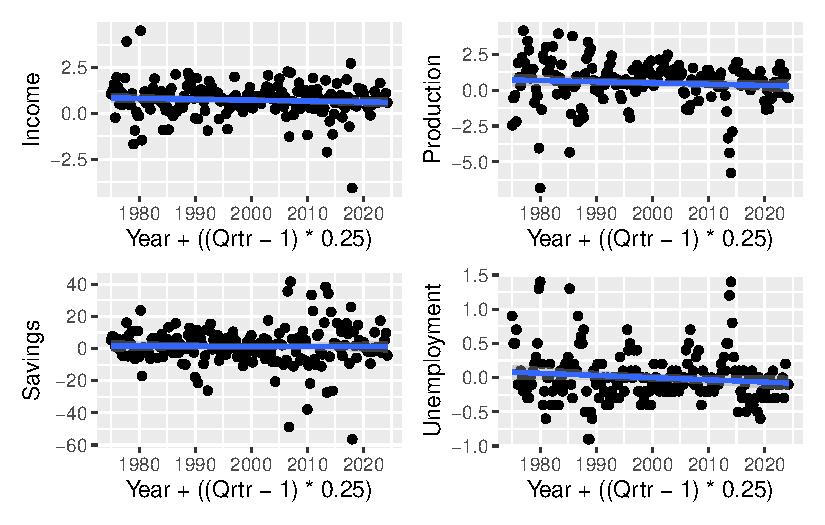
\includegraphics[keepaspectratio]{explanatory_predictions_files/figure-pdf/unnamed-chunk-2-1.pdf}}

\begin{Shaded}
\begin{Highlighting}[]
\NormalTok{vars\_lst }\OtherTok{\textless{}{-}} \FunctionTok{list}\NormalTok{(growth}\SpecialCharTok{$}\NormalTok{Income, growth}\SpecialCharTok{$}\NormalTok{Production, growth}\SpecialCharTok{$}\NormalTok{Savings, growth}\SpecialCharTok{$}\NormalTok{Unemployment)}

\ControlFlowTok{for}\NormalTok{ (i }\ControlFlowTok{in} \DecValTok{1}\SpecialCharTok{:}\DecValTok{4}\NormalTok{)\{}\FunctionTok{acf}\NormalTok{(vars\_lst[[i]])\}}
\end{Highlighting}
\end{Shaded}

\pandocbounded{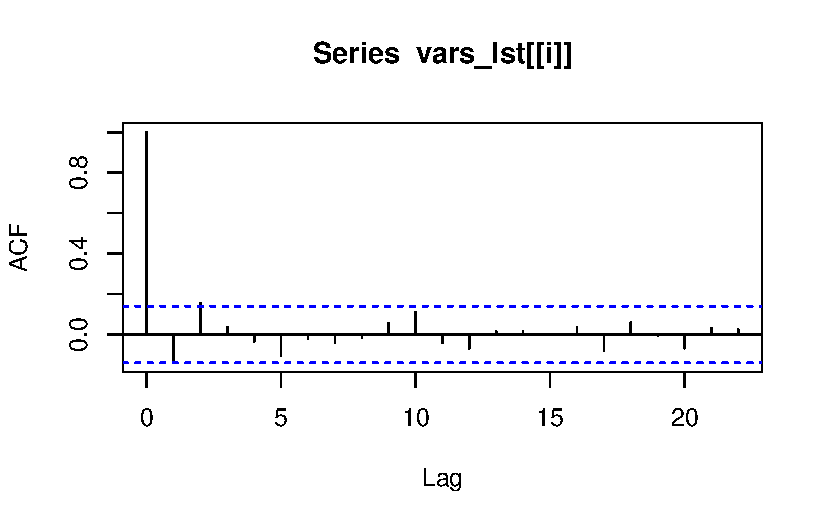
\includegraphics[keepaspectratio]{explanatory_predictions_files/figure-pdf/unnamed-chunk-3-1.pdf}}

\pandocbounded{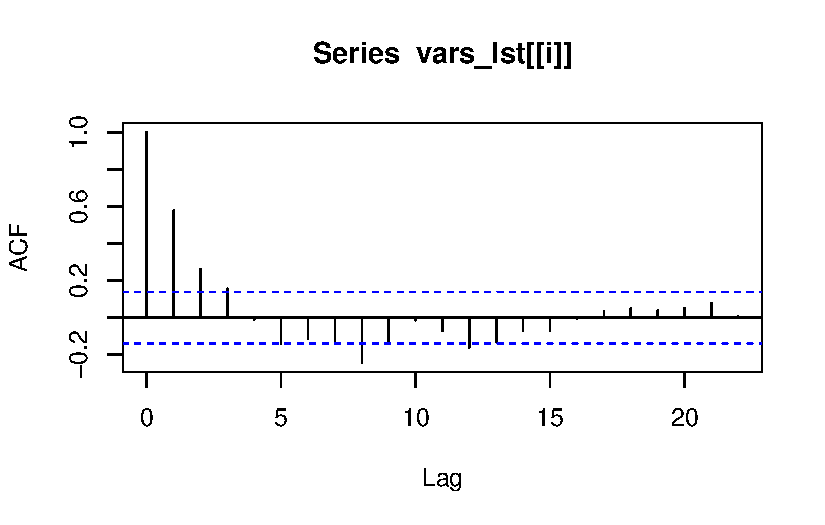
\includegraphics[keepaspectratio]{explanatory_predictions_files/figure-pdf/unnamed-chunk-3-2.pdf}}

\pandocbounded{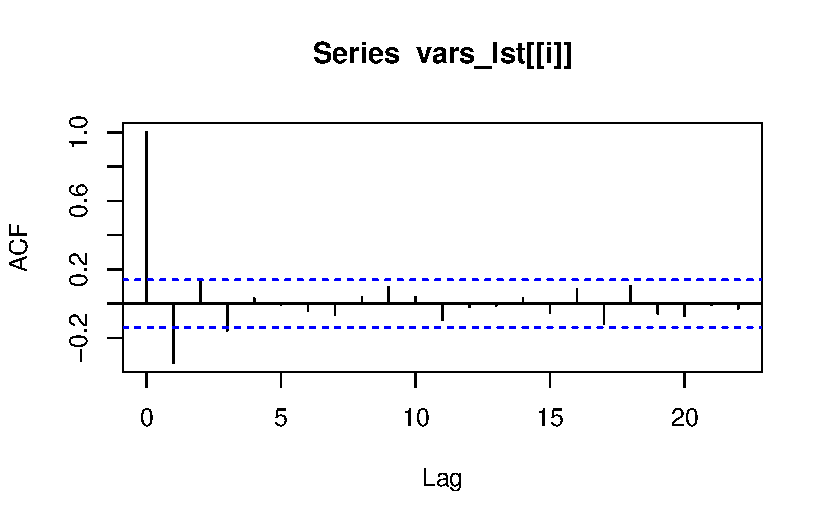
\includegraphics[keepaspectratio]{explanatory_predictions_files/figure-pdf/unnamed-chunk-3-3.pdf}}

\pandocbounded{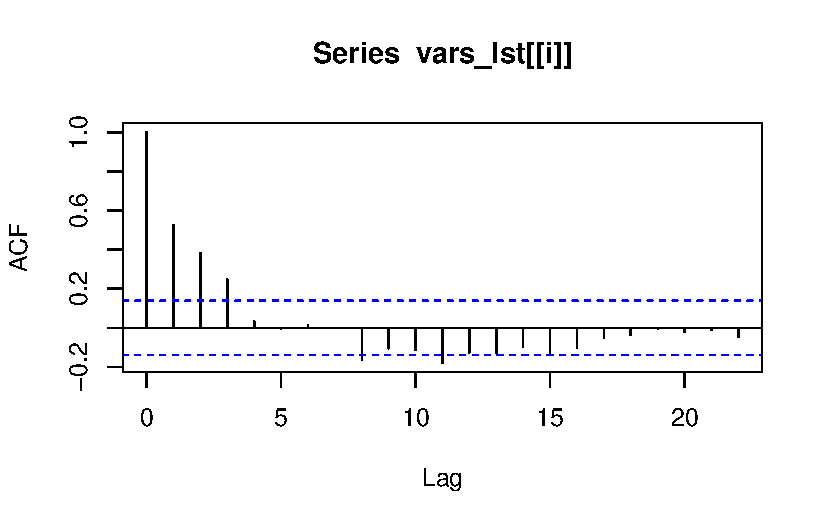
\includegraphics[keepaspectratio]{explanatory_predictions_files/figure-pdf/unnamed-chunk-3-4.pdf}}

\begin{Shaded}
\begin{Highlighting}[]
\CommentTok{\# Predict only Q1 2025 (i.e., 2025{-}01{-}01)}
\NormalTok{future\_2025 }\OtherTok{\textless{}{-}} \FunctionTok{tibble}\NormalTok{(}\AttributeTok{ds =} \FunctionTok{as.Date}\NormalTok{(}\StringTok{"2025{-}01{-}01"}\NormalTok{))}
\end{Highlighting}
\end{Shaded}

\begin{Shaded}
\begin{Highlighting}[]
\CommentTok{\# Convert Year + Qrtr to a proper quarterly date (first day of the quarter)}
\NormalTok{grow\_prod }\OtherTok{\textless{}{-}}\NormalTok{ growth }\SpecialCharTok{\%\textgreater{}\%}
  \FunctionTok{mutate}\NormalTok{(}
    \AttributeTok{month =}\NormalTok{ (Qrtr }\SpecialCharTok{{-}} \DecValTok{1}\NormalTok{) }\SpecialCharTok{*} \DecValTok{3} \SpecialCharTok{+} \DecValTok{1}\NormalTok{,                     }\CommentTok{\# 1, 4, 7, 10}
    \AttributeTok{ds =} \FunctionTok{as.Date}\NormalTok{(}\FunctionTok{paste}\NormalTok{(Year, month, }\DecValTok{1}\NormalTok{, }\AttributeTok{sep =} \StringTok{"{-}"}\NormalTok{))}
\NormalTok{  ) }\SpecialCharTok{\%\textgreater{}\%}
  \FunctionTok{select}\NormalTok{(ds, }\AttributeTok{y =}\NormalTok{ Production)}

\CommentTok{\# Fit Prophet}
\NormalTok{proph\_prod }\OtherTok{\textless{}{-}} \FunctionTok{prophet}\NormalTok{(grow\_prod)}
\end{Highlighting}
\end{Shaded}

\begin{verbatim}
Disabling weekly seasonality. Run prophet with weekly.seasonality=TRUE to override this.
\end{verbatim}

\begin{verbatim}
Disabling daily seasonality. Run prophet with daily.seasonality=TRUE to override this.
\end{verbatim}

\begin{Shaded}
\begin{Highlighting}[]
\NormalTok{prod\_pred }\OtherTok{\textless{}{-}} \FunctionTok{predict}\NormalTok{(proph\_prod, future\_2025)}\SpecialCharTok{$}\NormalTok{yhat}

\NormalTok{prod\_pred}
\end{Highlighting}
\end{Shaded}

\begin{verbatim}
[1] 0.3172247
\end{verbatim}

\begin{Shaded}
\begin{Highlighting}[]
\CommentTok{\# Convert Year + Qrtr to a proper quarterly date (first day of the quarter)}
\NormalTok{grow\_inc }\OtherTok{\textless{}{-}}\NormalTok{ growth }\SpecialCharTok{\%\textgreater{}\%}
  \FunctionTok{mutate}\NormalTok{(}
    \AttributeTok{month =}\NormalTok{ (Qrtr }\SpecialCharTok{{-}} \DecValTok{1}\NormalTok{) }\SpecialCharTok{*} \DecValTok{3} \SpecialCharTok{+} \DecValTok{1}\NormalTok{,                     }\CommentTok{\# 1, 4, 7, 10}
    \AttributeTok{ds =} \FunctionTok{as.Date}\NormalTok{(}\FunctionTok{paste}\NormalTok{(Year, month, }\DecValTok{1}\NormalTok{, }\AttributeTok{sep =} \StringTok{"{-}"}\NormalTok{))}
\NormalTok{  ) }\SpecialCharTok{\%\textgreater{}\%}
  \FunctionTok{select}\NormalTok{(ds, }\AttributeTok{y =}\NormalTok{ Income)}

\CommentTok{\# Fit Prophet}
\NormalTok{proph\_inc }\OtherTok{\textless{}{-}} \FunctionTok{prophet}\NormalTok{(grow\_inc)}
\end{Highlighting}
\end{Shaded}

\begin{verbatim}
Disabling weekly seasonality. Run prophet with weekly.seasonality=TRUE to override this.
\end{verbatim}

\begin{verbatim}
Disabling daily seasonality. Run prophet with daily.seasonality=TRUE to override this.
\end{verbatim}

\begin{Shaded}
\begin{Highlighting}[]
\NormalTok{inc\_pred }\OtherTok{\textless{}{-}} \FunctionTok{predict}\NormalTok{(proph\_inc, future\_2025)}\SpecialCharTok{$}\NormalTok{yhat}

\NormalTok{inc\_pred}
\end{Highlighting}
\end{Shaded}

\begin{verbatim}
[1] 0.6129535
\end{verbatim}

\begin{Shaded}
\begin{Highlighting}[]
\CommentTok{\# Convert Year + Qrtr to a proper quarterly date (first day of the quarter)}
\NormalTok{grow\_sav }\OtherTok{\textless{}{-}}\NormalTok{ growth }\SpecialCharTok{\%\textgreater{}\%}
  \FunctionTok{mutate}\NormalTok{(}
    \AttributeTok{month =}\NormalTok{ (Qrtr }\SpecialCharTok{{-}} \DecValTok{1}\NormalTok{) }\SpecialCharTok{*} \DecValTok{3} \SpecialCharTok{+} \DecValTok{1}\NormalTok{,                     }\CommentTok{\# 1, 4, 7, 10}
    \AttributeTok{ds =} \FunctionTok{as.Date}\NormalTok{(}\FunctionTok{paste}\NormalTok{(Year, month, }\DecValTok{1}\NormalTok{, }\AttributeTok{sep =} \StringTok{"{-}"}\NormalTok{))}
\NormalTok{  ) }\SpecialCharTok{\%\textgreater{}\%}
  \FunctionTok{select}\NormalTok{(ds, }\AttributeTok{y =}\NormalTok{ Savings)}

\CommentTok{\# Fit Prophet}
\NormalTok{proph\_sav }\OtherTok{\textless{}{-}} \FunctionTok{prophet}\NormalTok{(grow\_sav)}
\end{Highlighting}
\end{Shaded}

\begin{verbatim}
Disabling weekly seasonality. Run prophet with weekly.seasonality=TRUE to override this.
\end{verbatim}

\begin{verbatim}
Disabling daily seasonality. Run prophet with daily.seasonality=TRUE to override this.
\end{verbatim}

\begin{Shaded}
\begin{Highlighting}[]
\NormalTok{sav\_pred }\OtherTok{\textless{}{-}} \FunctionTok{predict}\NormalTok{(proph\_sav, future\_2025)}\SpecialCharTok{$}\NormalTok{yhat}

\NormalTok{sav\_pred}
\end{Highlighting}
\end{Shaded}

\begin{verbatim}
[1] 2.320703
\end{verbatim}

\begin{Shaded}
\begin{Highlighting}[]
\CommentTok{\# Convert Year + Qrtr to a proper quarterly date (first day of the quarter)}
\NormalTok{grow\_unem }\OtherTok{\textless{}{-}}\NormalTok{ growth }\SpecialCharTok{\%\textgreater{}\%}
  \FunctionTok{mutate}\NormalTok{(}
    \AttributeTok{month =}\NormalTok{ (Qrtr }\SpecialCharTok{{-}} \DecValTok{1}\NormalTok{) }\SpecialCharTok{*} \DecValTok{3} \SpecialCharTok{+} \DecValTok{1}\NormalTok{,                     }\CommentTok{\# 1, 4, 7, 10}
    \AttributeTok{ds =} \FunctionTok{as.Date}\NormalTok{(}\FunctionTok{paste}\NormalTok{(Year, month, }\DecValTok{1}\NormalTok{, }\AttributeTok{sep =} \StringTok{"{-}"}\NormalTok{))}
\NormalTok{  ) }\SpecialCharTok{\%\textgreater{}\%}
  \FunctionTok{select}\NormalTok{(ds, }\AttributeTok{y =}\NormalTok{ Unemployment)}

\CommentTok{\# Fit Prophet}
\NormalTok{proph\_unem }\OtherTok{\textless{}{-}} \FunctionTok{prophet}\NormalTok{(grow\_unem)}
\end{Highlighting}
\end{Shaded}

\begin{verbatim}
Disabling weekly seasonality. Run prophet with weekly.seasonality=TRUE to override this.
\end{verbatim}

\begin{verbatim}
Disabling daily seasonality. Run prophet with daily.seasonality=TRUE to override this.
\end{verbatim}

\begin{Shaded}
\begin{Highlighting}[]
\NormalTok{unem\_pred }\OtherTok{\textless{}{-}} \FunctionTok{predict}\NormalTok{(proph\_unem, future\_2025)}\SpecialCharTok{$}\NormalTok{yhat}

\NormalTok{unem\_pred}
\end{Highlighting}
\end{Shaded}

\begin{verbatim}
[1] -0.1215834
\end{verbatim}




\end{document}
